 
\usepackage[a4paper, twocolumn]{geometry} 
\usepackage{tikz}
\usepackage[utf8]{inputenc}
\usepackage{amsmath}
\usepackage{amsfonts}
\usepackage{amssymb}
\usepackage{stackrel}
%\usepackage{kpfonts}
\usepackage{amssymb, amsmath, amsbsy} 
\usepackage{makeidx}
\usepackage{graphicx}
\usepackage{multicol}
\usepackage{changepage}
\usepackage{float}
\usepackage{cite}
\usepackage{lipsum}
\usepackage{pstricks, caption}
\usepackage{url}
\usepackage[spanish, es-tabla]{babel}
\usepackage[shortlabels]{enumitem}
\usepackage{longtable,multirow,booktabs}
\usepackage{rotating}
\usepackage{caption}
\usepackage{multirow, array}
\usepackage{anyfontsize}
\usepackage{fix-cm}
\usepackage{calligra}
\usepackage{mathptmx}
\usepackage{caption}
\usepackage{fancyvrb}
%\usepackage{esvect}
\usepackage{xargs}
\usepackage{subfigure} 
\usepackage {titletoc}
\usepackage[T1]{fontenc}
%\usepackage[hyphens]{url}
\usepackage[breaklinks,colorlinks=true,linkcolor=blue,citecolor=red, urlcolor=blue]{hyperref}
\usepackage{flushend}

\documentclass[13,twocolumn,letterpaper]{article}
    \usepackage[spanish,english]{babel}
    \usepackage[utf8x]{inputenc}
    \usepackage[T1]{fontenc}
    \usepackage[a4paper,top=3cm,bottom=2cm,left=3cm,right=3cm,marginparwidth=1.75cm]{geometry}
    \usepackage{amsmath}
    \usepackage[colorinlistoftodos]{todonotes}
    \usepackage[colorlinks=true, allcolors=blue]{hyperref}
    \usepackage{float}
    
    
 \spanishdecimal{.}
\renewcommand{\figurename}{\textbf{Figura}}
\renewcommand{\tablename}{\textbf{Tabla}}
\renewcommand{\refname}{Bibliografía}
\renewcommand{\abstractname}{\large\textbf{Resumen}}
\renewcommand{\contentsname}{Contenido}
\renewcommand{\partname}{Parte}
\renewcommand{\appendixname}{Apéndice}
\renewcommand{\sin}{sen}	
\newenvironment{Figure}{\par\medskip\noindent\minipage{\linewidth}}{\endminipage\par\medskip}

    
    \title{
    		%\vspace{-1in} 	
    		\usefont{OT1}{bch}{b}{n}
    		\normalfont \normalsize \textsc{INSTITUTO POLITÉCNICO NACIONAL \\ 
    		ESCUELA SUPERIOR DE FISICA Y MATEMATICAS \\
    		ACADEMIA DE FÍSICA EXPERIMENTAL} \\ 
    		FÍSICA IV: LABORATORIO DE ÓPTICA. \\[10pt]
    		\huge Práctica IV - A :\\
    Formación de Imágenes con Lentes Delgadas.\\
    }
    
    \usepackage{authblk}
    \author[0]{Alumno: Flores Rodriguez Jaziel David \\
    Boleta: 2014030429 \\
    Profesor: Dr. Janos Zsargo\\
    Grupo: 4FV2-B \\
            }
    \begin{document}
    
    \maketitle
   
    \selectlanguage{spanish}
    
    \section*{Resumen}
    El objetivo principal de este reporte es el de dar a conocer los resultados obtenidos al estudiar la formación de imágenes con lentes delgadas, para establecer los resultados aquí presentados se  realizó un experimento en el cual mediante el empleo de una lente delgada positiva de $f$ conocida, localizamos las imágenes reales de objetos reales. \\\\
	Palabras clave: \emph{ecuación de magnificación, lentes delgadas, imágenes, ecuación de Gauss, ecuación de Newton} \\ 

\section*{Introducción }
{ 
	\begin{figure*}[ht!]
		\centering
		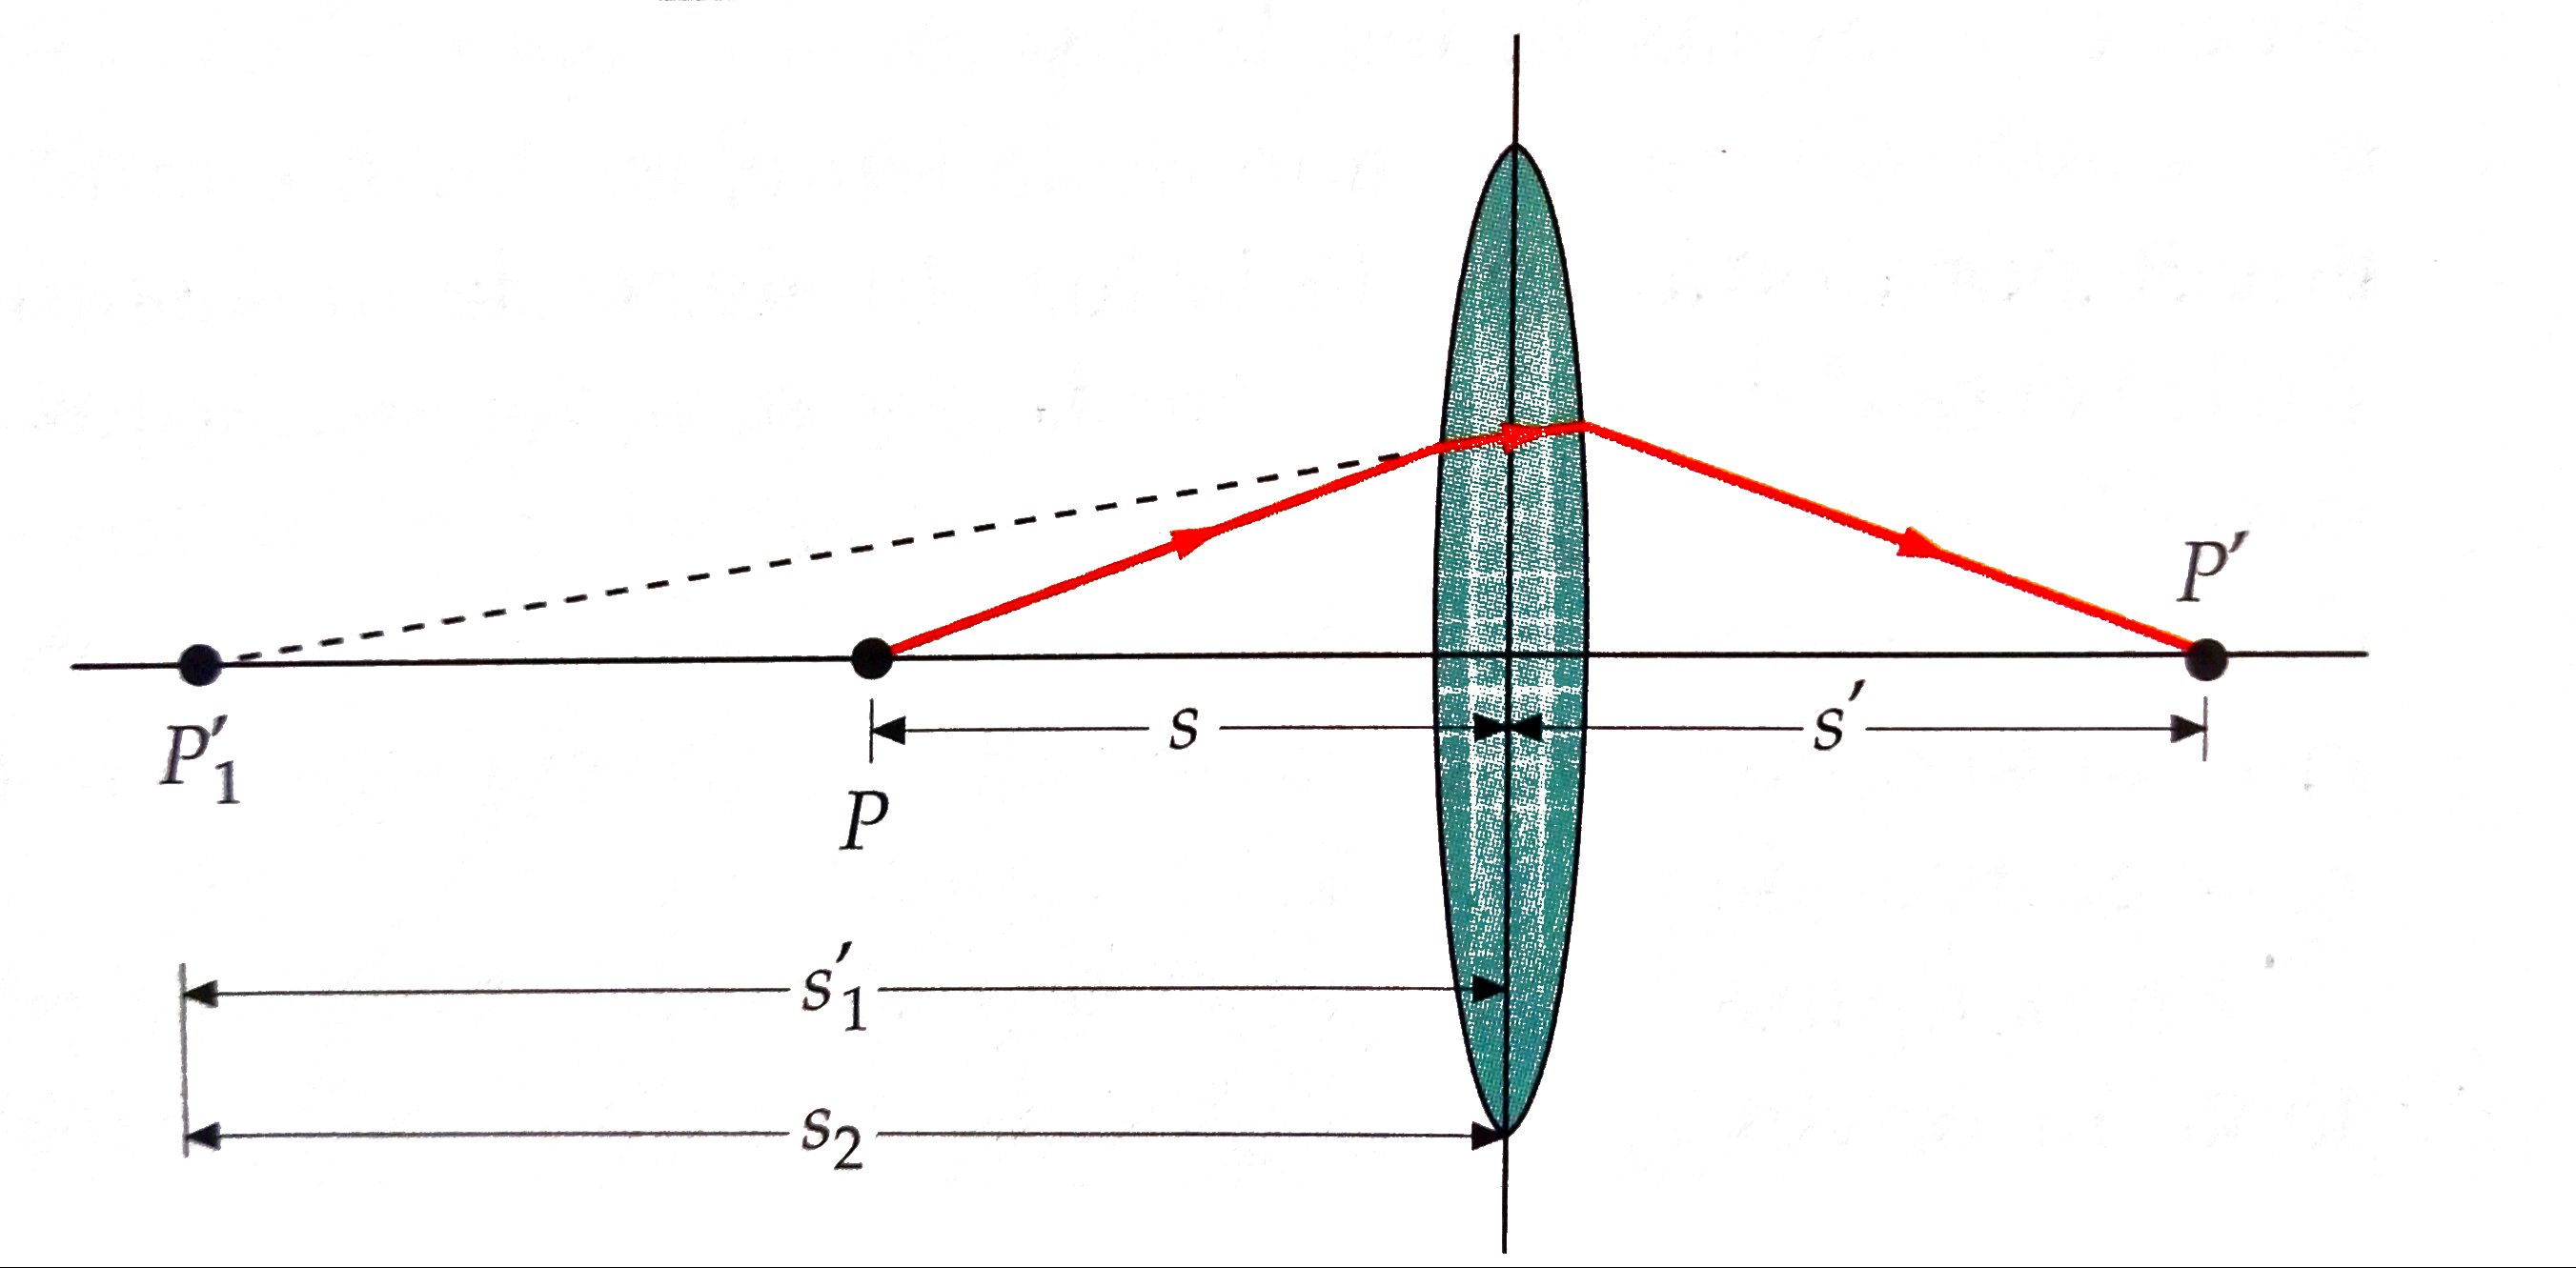
\includegraphics[width=\linewidth]{fig1}
		\caption[Fig 1]{\footnotesize{La refracción en la primera superficie origina una imagen virtual en $P_{1}'$. Los rayos inciden sobre la segunda superficie como si provinieran de $P_{1}'$.}}
		\label{fig:fig-1}
	\end{figure*}
	
	En un arreglo como el de la Figura 1 sabemos que se cumple la ecuación 
	\begin{equation}\label{ec1}
		\dfrac{1}{s}+\dfrac{1}{s'}=\left(\dfrac{n}{n_{aire}}-1\right)\left(\dfrac{1}{r_{1}}-\dfrac{1}{r_{2}}\right)
	\end{equation}
	La ecuación anterior de la distancia imagen $s'$ en función de la distancia objeto $s$ y de las propiedades de la lente delgada ($r_{1}$, $r_{2}$ y su indice de refracción $n$). La distancia focal $f$ de una lente delgada se define como la distancia imagen que corresponde a una distancia objeto infinita. Haciendo $s$ igual a infinito y escribiendo $f$ en lugar de la distancia imagen $s'$, se tiene 
	\begin{equation}\label{ec2}
		\dfrac{1}{f}=\left(\dfrac{n}{n_{aire}}-1\right)\left(\dfrac{1}{r_{1}}-\dfrac{1}{r_{2}}\right)
	\end{equation}
	La ecuación anterior se conoce como la \textbf{fórmula del fabricante de lentes}; la cual nos da la distancia focal de una lente delgada en función de sus propiedades. Sustituyendo el segundo miembro de la ecuación (\ref{ec1}) por $\dfrac{1}{f}$, se tiene 
	
	\begin{equation}\label{ec3}
		\dfrac{1}{f}=\dfrac{1}{s}+\dfrac{1}{s'}	
	\end{equation}
	que se denomina \textbf{ecuación de la lente delgada} ó \textbf{ecuación de Gauss}.
	\subsection*{Ecuación de Gauss, y ecuación de magnificación}
	{
		Se tiene el siguiente arreglo:
		\begin{figure}[!htb]
			\centering
			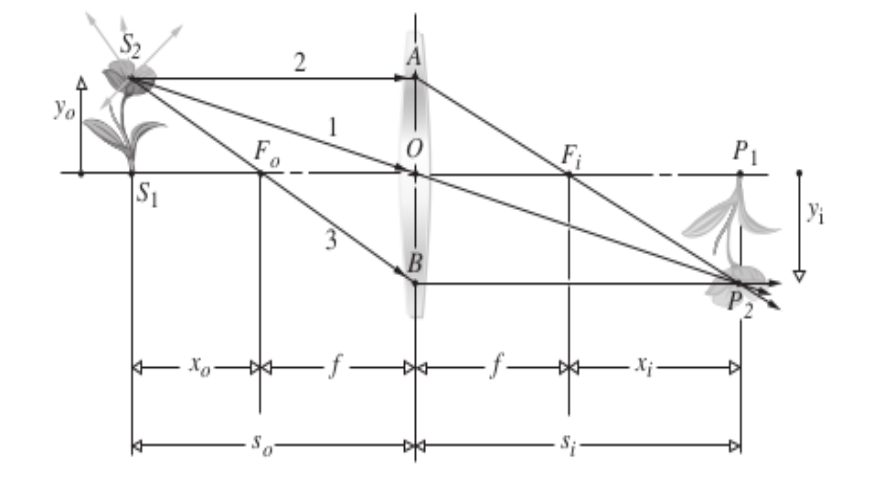
\includegraphics[width=0.5\textwidth]{./fig2}
			\caption[Fig 1]{\footnotesize{Arreglo para la demostración de la ecuación de Gauss, y ecuación de magnificación}}
			\label{fig:fig-2}
		\end{figure}	
	\\Observe que los triángulos $\triangle AOF_{i}$ y \\$\triangle P_{2}P_{1}F_{i}$ son congruentes, es decir 
	\begin{equation}\label{ec4}
		\dfrac{y_{o}}{|y_{i}|}=\dfrac{f}{(s_{i}-f)}
	\end{equation}
	del mismo modo, los triángulos $\triangle S_{2}S_{1}O\;$ y $\;\triangle P_{2}P_{1}O\;$ son congruentes y 
	\begin{equation}\label{ec5}
		\dfrac{y_{o}}{|y_{i}|}=\dfrac{s_{o}}{s_{i}}
	\end{equation}
	de acuerdo a la convención de signos estándar se tiene que $y_{i}>0$ por lo tanto combinando las ecuaciones (\ref{ec4}) y (\ref{ec5})
	obtenemos
	\begin{equation}\label{ec6}
		\dfrac{s_{o}}{s_{i}}=\dfrac{f}{(s_{i}-f)}
	\end{equation} 
	y 
	$$\dfrac{1}{f}=\dfrac{1}{s_{o}}+\dfrac{1}{s_{i}}$$
	que no es más que la ecuación (\ref{ec3}) pero adaptada a la notación de la figura 2. \\
	Además, los triángulos $\triangle S_{2}S_{1}F_{o}\;$ y $\;\triangle BOF_{o}$ son congruentes y
	\begin{equation}\label{ec7}
		\dfrac{f}{(s_{o}-f)}=\dfrac{|y_{i}|}{y_{o}}
	\end{equation}
	Usando las distancias medidas desde los puntos focales se obtiene claramente 
	\begin{equation}\label{ec8}
		x_{o}=s_{o}-f\atop
		x_{i}=s_{i}-f
	\end{equation}
	 y combinando la ecuación (\ref{ec4}) con la ecuación (\ref{ec7}) se tiene:
	$$\dfrac{f}{(s_{i}-f)}=\dfrac{(s_{o}-f)}{f}$$
	O bien
	
	\begin{equation}\label{ec9}
		f^{2}=(s_{o}-f)(s_{i}-f)
	\end{equation}
	
	Sustituyendo el sistema de ecuaciones (\ref{ec8}) en la ecuación (\ref{ec9}) optemos finalmente 
	\begin{equation}\label{ec10}
		f^{2}=x_{o}x_{i}
	\end{equation}
	La cual recibe el nombre de \textbf{ecuación de lentes forma Newtoniana}.\\
	De la ecuación (\ref{ec7}) se obtiene el aumento lateral 
	$$m\equiv\dfrac{y_{i}}{y_{o}}$$
	teniendo en cuenta la ecuación (\ref{ec5}) se obtiene 
	\begin{equation}\label{ec11}
		m=-\dfrac{s_{i}}{s_{o}}
	\end{equation}
	que es la \textbf{ecuación de magnificación}.
	}
}
\newpage
\onecolumn

\section*{Experimentos}
{
	Para el caso en el que las lentes fueron positivas se monto el experimento como se muestra en la figura \ref{fig:fig-3}
	\begin{figure}[!htb]
		\centering
		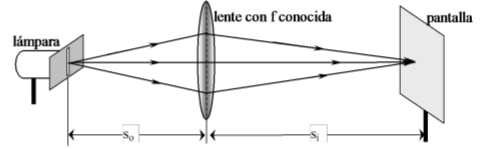
\includegraphics[width=0.5\textwidth]{./fig3}
		\caption[Fig 1]{\footnotesize{Montaje experimental para lentes positivas.}}
		\label{fig:fig-3}
	\end{figure}
	\\Posteriormente mediante el empleo de una lente delgada positiva de $f$ conocida, se localizó las imágenes reales de
	objetos reales y se registraron los datos en la tabla 1, y la tabla 2 dichas tablas están en la sección de datos obtenidos, los resultados obtenidos así como los ajustes y graficas están en la sección de resultados obtenidos.\\
	Para lentes negativas nos auxiliamos de una lente positiva para medir la parte de la hipérbola con imagen real, las mediciones efectuadas se registraron en las tablas 3 y 4  las cuales se encuentran en la sección de datos obtenidos, los ajustes están en la sección de resultados obtenidos. El montaje experimental se muestra en la figura \ref{fig:fig-4}.
	\begin{figure}[!htb]
		\centering
		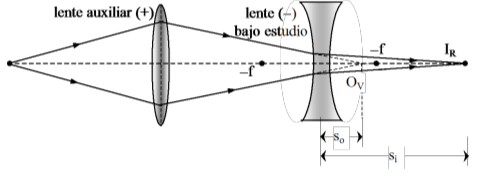
\includegraphics[width=0.5\textwidth]{./fig4}
		\caption[Fig 1]{\footnotesize{Montaje experimental para lentes positivas.}}
		\label{fig:fig-4}
	\end{figure}
}


\section*{Datos obtenidos}

		En las tablas se registraron los siguientes datos: $s_{o}$, $s_{i}$, $x_{o}$ y $x_{i}$, los cuales se obtiene de las siguientes formulas
	$$ s_{o}=f+x_{o}\;\;\;\;\;\;\;
	\;\;\;s_{i}=f+x_{i}$$
	$$x_{o}=s_{o}-f \;\;\;\;\;\;\;
	\;\;\;
	x_{i}=s_{i}-f	$$
	Para lentes positivas se realizaron 10 mediciones con dos diferentes lentes cuyas $f$ eran de $100 \; mm$ y $200\; mm$, y para lenes negativas solo se realizaron 3 mediciones.\\
	Para la lente positiva de $200\; mm$ los datos obtenidos son los siguientes:
		 


\begin{table}[htb]
	\centering
	\begin{tabular}{|| c | c | c | c | c | c | c | c | c ||}
\hline \hline 
		N & $s_{o}$ ($cm$) & $s_{i}$ ($cm$) & $x_{o}$  ($cm$) & $x_{i}$ ($cm$) & $m$ & Objeto & Imagen & Orientación \\ \hline \hline
		1 &  120  & 24.5  & 100   & 4.5  & 0.20 &  0.57  & 0.18 & Invertida \\
		2 &  85   & 27    & 65    & 7    & 0.31 &  0.57  & 0.25 & Invertida \\
		3 &  80   & 27.2  & 60    & 7.2  & 0.34 &  0.57  & 0.30 & Invertida\\
		4 & 70.05 & 28.95 & 50.05 & 8.95 & 0.41 &  0.57  & 0.34 & Invertida \\
		5 &  60.6 & 30.7  & 40.6  & 10.7 & 0.50 &  0.57  & 0.37 & Invertida \\
		6 &  54.1 & 32.4  & 34.1  & 12.4 & 0.59 &  0.57  & 0.42 & Invertida\\
		7 &  40.5 & 39.5  & 20.5  & 19.5 & 0.97 &  0.57  & 0.59 & Invertida  \\
		8 &  35   & 47.5  & 15    & 27.5 & 1.35 &  0.57  & 0.76 & Invertida\\
		9 &  31.8 & 54.5  & 11.8  & 34.5 & 1.72 &  0.57  & 0.96 & Invertida \\
		10 & 26.1 & 85.9  & 6.1   & 65.9 & 3.2  &  0.57  & 1.70 & Invertida \\ \hline
	\end{tabular}
	\caption{Datos obtenidos en el experimento con lentes positivas con $f=200\;mm$} \label{tabla1}
\end{table}


\begin{table}[htb]
	\centering
	\begin{tabular}{|| c | c | c | c | c | c | c | c | c ||} 
	\hline \hline
		N & $s_{o}$ ($cm$) & $s_{i}$ ($cm$) & $x_{o}$  ($cm$) & $x_{i}$ ($cm$) & $m$ & Objeto & Imagen & Orientación \\ \hline \hline
		1 & -15 & 6.8	 & -35 	& 13.2 	& 0.45 & 0.88  	& 0.44 & Derecha \\
		2 &  -16	 & 7 	 & -36 	& -13 	& 0.43 & 0.92 	& 0.5 & Derecha \\
		3 &   -14.5 & 6.5  & -34.5 	& -12.8 	& 0.44 & 0.85 	& 0.4 & Derecha \\ \hline
	\end{tabular}
	\caption{Datos obtenidos en el experimento con lentes positivas con $f=200\;mm$ con $s_{o}<0$} \label{tabla2}
\end{table}


\begin{table}[h]
\centering 
\begin{tabular}{|| c | c | c | c | c | c | c | c | c ||}
\hline \hline
	N & $s_{o}$ ($cm$) & $s_{i}$ ($cm$) & $x_{o}$  ($cm$) & $x_{i}$ ($cm$) & $m$ & Objeto & Imagen & Orientación  \\
\hline \hline 
	1 &  45 	& 13.2 	& 35 	& 3.2	& 0.29 & 0.57  & 0.25 & Invertida   \\
	2 &  40 	& 14.2 	& 30 	& 4.2	& 0.35	& 0.57  & 0.33 & Invertida   \\
	3 &  35 	& 14.8 	& 25 	& 4.8	& 0.42	& 0.57  & 0.27 & Invertida   \\
	4 &  30 	& 15.9 	& 20 	& 5.9	& 0.53	& 0.57  & 0.31 & Invertida   \\
	5 &  25 	& 17.2 	& 15 	& 7.2	& 0.68	& 0.57  & 0.42 & Invertida   \\
	6 &  20 	& 20.5 	& 10 	& 10.5	& 1.02	& 0.57  & 0.59 & Invertida   \\
	7 &  17.5 	& 23.4 	& 7.5 	& 13.4 	& 1.33	& 0.57  & 0.77 & Invertida   \\
	8 &  15 	& 29.9 	& 5 	& 19.9	& 1.99	& 0.57  & 1.06 & Invertida   \\ 
	9 &  13.2 	& 39.4 	& 3.2 	& 29.4	& 2.98	& 0.57  & 1.58 & Invertida   \\
	10 &  12.4 	& 48.7 	& 2.4 	& 38.7	& 3.92	& 0.57  & 2.06 & Invertida   \\\hline
\end{tabular}
\caption{Datos obtenidos en el experimento con lentes positivas con $f=100\;mm$} 
\end{table}


\begin{table}[h]
\centering
\begin{tabular}{|| c | c | c | c | c | c | c | c | c ||}
\hline \hline
	N & $s_{o}$ ($cm$) & $s_{i}$ ($cm$) & $x_{o}$  ($cm$) & $x_{i}$ ($cm$) & $m$ & Objeto & Imagen & Orientación  \\
\hline \hline
1 & -11 & 5.5	 & -21 	& -4.5 	& -0.5 & 0.67  	& 0.35 & Derecha \\
2 &  -10.5	 & 5.3 	 & -20.5 	& -4.7 	& -0.504 &  0.6	& 0.31 & Derecha \\
3 &   -10 & 5  & -20 	& -5 	& -0.5 & 0.57 	& 0.29 & Derecha \\ \hline
\end{tabular}
	\caption{Datos obtenidos en el experimento con lentes positivas con $f=100\;mm$ con  $s_{o}<0$} \label{tabla4}
\end{table}

\begin{table}[h]
\centering
\begin{tabular}{|| c | c | c | c | c | c | c | c | c ||}
\hline \hline
	N & $s_{o}$ ($cm$) & $s_{i}$ ($cm$) & $x_{o}$  ($cm$) & $x_{i}$ ($cm$) & $m$ & Objeto & Imagen & Orientación  \\
	\hline \hline
	1	& -6	&	  9.7	& -26.0 	& -0.3	& -1.6	&	3.24	&	4.3		&	Derecha	\\
	2	& -6.7	&	 11.6	& -26.7		& 1.6	& -1.73	&	2.28	&	3.02	&   Derecha	\\
	3	& -7.1	&	 11.4	& -27.1		& 1.4	& -1.6	&	2.46	&	3.22	&   Derecha	\\\hline \hline
\end{tabular} 
	\caption{Datos obtenidos en el experimento con lentes  negativas con $f=100\;mm$} 
\end{table}

\begin{multicols}{2}
\pagebreak
\twocolumn
	\section*{Resultados obtenidos}
	{	
		La representación grafica para los datos de las tablas \ref{tabla1} y \ref{tabla2} es la siguiente
		\begin{Figure}
			\centering
			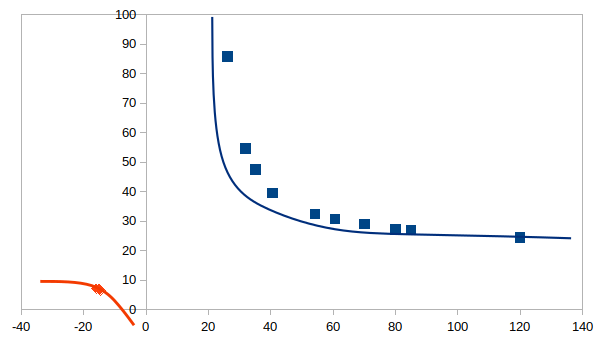
\includegraphics[width=\linewidth]{fig5}
			\caption{Gafica $s_{i}\;vs\;s_{o}$ de los datos de las tablas \ref{tabla1} y \ref{tabla2} en azul y anaranjado respectivamente.}
			}
			\label{fig:fig-5}
		\end{Figure}
		De la ecuación (\ref{ec3}) se tiene que 
		$$\dfrac{1}{f}=\dfrac{1}{s_{o}}+\dfrac{1}{s_{i}}$$
		proponiendo el siguiente cambio de variable 
		\begin{equation}\label{ec12}
			y=\dfrac{1}{s_{i}}\;\;\;\;\;x=\dfrac{1}{s_{o}}
		\end{equation}
		se tiene que 
		\begin{equation}\label{ec13}
			y=\dfrac{1}{f}-x
		\end{equation}
		de esta manera el ajuste que se obtuvo para los datos utilizando este cambio de variable es el siguiente 
		\begin{equation}\label{ec14}
			y=0.04861-0.9628x
		\end{equation}
		El comportamiento gráfico de los datos ajustados con el cambio de variable anterior es el siguiente  
		\begin{Figure}
			\centering
			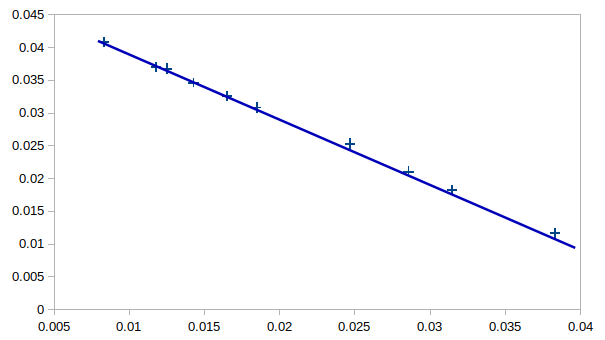
\includegraphics[width=\linewidth]{fig6}
			\caption{\footnotesize{Grafica de los datos de la tabla \ref{tabla1} despues de aplicarles el cambio de variable.}}
			\label{fig:fig-6}
		\end{Figure}
	luego la ecuación (\ref{ec14}) se reescribe como 
	\begin{equation}
		\dfrac{1}{s_{i}}+\dfrac{0.9628}{s_{o}}=\dfrac{1}{20.5718}
	\end{equation}
	para este caso se tenia que $f=20 \;cm$ entonces se obtuvo un error porcentual de 
	$$e\%=\dfrac{|20-20.5718|}{20}\times 100=2.85 \%$$
	este error porcentual es el obtenido al usar la ecuación guassiana de los lentes.\\
	Los resultados obtenidos utilizando la ecuación Newtoniana para los lentes (Ec. (\ref{ec10})) es la siguiente, su comportamiento gráfico  $x_{i}\;vs\;x_{o}$ es el siguiente
	\begin{Figure}
		\centering
		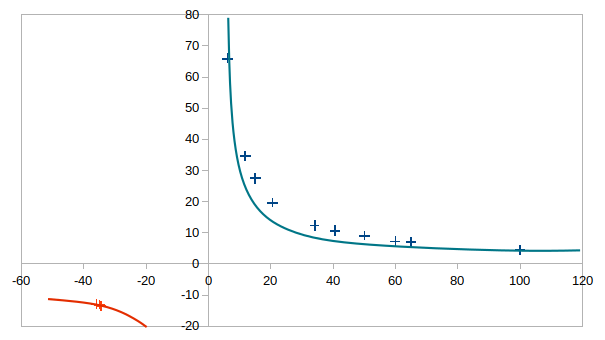
\includegraphics[width=\linewidth]{fig7}
		\caption{\footnotesize{Grafica de los $x_{i}\;vs\;x_{o}$ datos de las tablas \ref{tabla1} y \ref{tabla2} en azul y naranje respectivamente.}}
		\label{fig:fig-7}
	\end{Figure} 
	De la ecuación \ref{ec10} se tiene el siguiente cambio de variable 
	\begin{equation}\label{ec16}
		y=x_{i}\;\;\;\; x=\dfrac{1}{x_{o}}
	\end{equation} 
	Se obtiene la ecuación 
	\begin{equation}\label{ec17}
		y=f^{2}x
	\end{equation}  
	Utilizando este cambio de variable en los de la tabla 1 ($x_{i}\;vs\;x_{o}$) se obtuvo la siguiente ecuación de ajuste
	\begin{equation}\label{ec18}
		y=398.0443x+0.7243
	\end{equation} 
	El gráfico que representa la ecuación de ajuste anterior es el siguiente
	\begin{Figure}
		\centering
		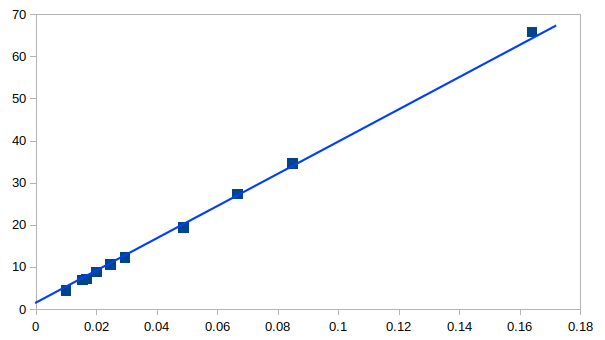
\includegraphics[width=\linewidth]{fig8}
		\caption{\footnotesize{Grafica de los $x_{i}\;vs\;x_{o}$ datos de la tabla \ref{tabla1} despues de ajustar con el cambio de variable propuesto en \ref{ec16}.}}
		\label{fig:fig-8}
	\end{Figure} 
de la ecuación (\ref{ec18}) se sigue que 
$$398.0443x=\dfrac{398.0443}{x_{o}}=\dfrac{f^{2}}{x_{o}}\implies f^{2}=398.0443$$
por lo tanto $f=19.9510\;cm$, utilizando la ecuación de Newton se obtuvo el siguiente porcentaje de error porcentual
$$e\%=\dfrac{|20-19.9510|}{20}\times 100=0.245 \%$$
Para la lente positiva de $f=100 \;mm$ los resultados son los siguientes, el gráfico de los datos de las tablas \ref{tabla3} y \ref{tabla4} esta en la figura \ref{fig:fig-9}
\begin{Figure}
	\centering
	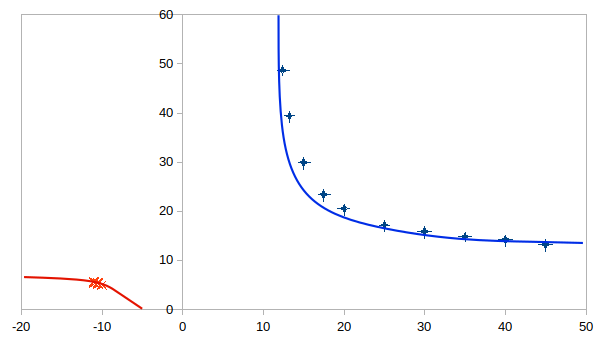
\includegraphics[width=\linewidth]{fig9}
	\caption{\footnotesize{Grafica de los $s_{i}\;vs\;s_{o}$ datos de las tablas \ref{tabla3} \ref{tabla4} en azul y naranja respectivamente.}}
	\label{fig:fig-9}
\end{Figure} 
 y la ecuación de ajuste utilizando el cambio de variable de \ref{ec12} es la siguiente 
\begin{equation}
	y=0.0941-0.9101x
\end{equation}
y el grafico comportamiento gráfico se puede observar en la figura \ref{fig:fig-10}
\begin{Figure}
	\centering
	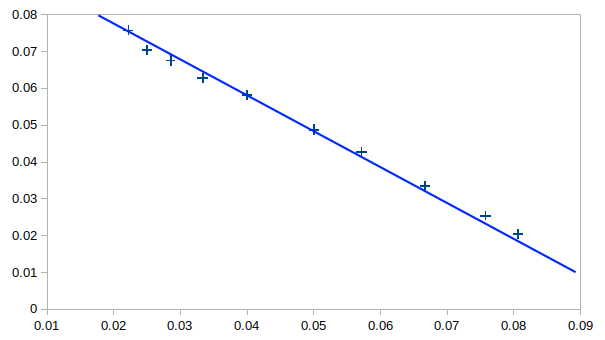
\includegraphics[width=\linewidth]{fig10}
	\caption{\footnotesize{Grafica de los $s_{i}\;vs\;s_{o}$ datos de la tabla \ref{tabla1} despues de ajustar con el cambio de variable propuesto en \ref{ec12}.}}
	\label{fig:fig-10}
\end{Figure} 

luego la ecuación (\ref{ec14}) se reescribe como 
\begin{equation}
\dfrac{1}{s_{i}}+\dfrac{0.9101}{s_{o}}=\dfrac{1}{10.6269}
\end{equation}
para este caso se tenia que $f=10 \;cm$ entonces se obtuvo un error porcentual de 
$$e\%=\dfrac{|10-10.6269|}{10}\times 100= 6.269\%$$
este erro porcentual es el obtenido al usar la ecuación guassiana de los lentes.\\
Los resultados obtenidos mediante la ecuación (\ref{ec10}) se presenta a continuación, el grafico $x_{i}\;vs\;x_{o}$ es el siguiente
\begin{Figure}
	\centering
	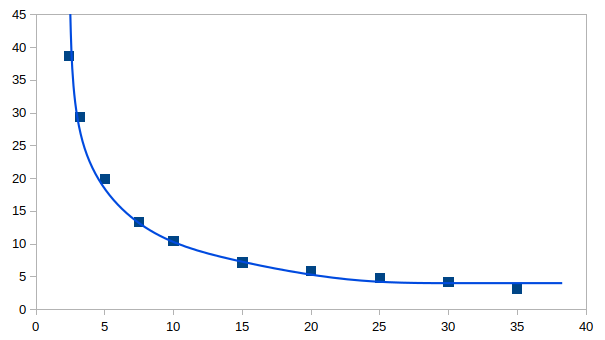
\includegraphics[width=\linewidth]{fig11}
	\caption{\footnotesize{Grafica de los $s_{i}\;vs\;s_{o}$ datos de la tabla \ref{tabla1} despues de ajustar con el cambio de variable propuesto en \ref{ec12}.}}
	\label{fig:fig-11}
\end{Figure} 
Mediante el cambio de variable propuesto en (\ref{ec12}) se obtuvo la siguiente ecuación
\begin{equation}\label{ec21}
y=90.5604x+1.2129
\end{equation}
 y la gráfica después de realizar este ajuste es la siguiente
	\begin{Figure}
	\centering
	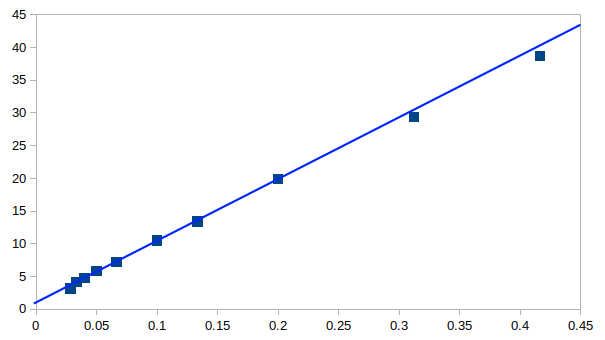
\includegraphics[width=\linewidth]{fig12}
	\caption{\footnotesize{Grafica de los $x_{i}\;vs\;x_{o}$ datos de la tabla \ref{tabla1} despues de ajustar con el cambio de variable propuesto en \ref{ec16}.}}
	\label{fig:fig-12}
\end{Figure} 
Luego de la ecuación (\ref{ec18}) se sigue que 
$$90.5604x=\dfrac{90.5604}{x_{o}}=\dfrac{f^{2}}{x_{o}}\implies f^{2}=90.5604$$
por lo tanto $f=9.5163\;cm$, utilizando la ecuación de Newton se obtuvo el siguiente porcentaje de error porcentual
$$e\%=\dfrac{|10-9.5163|}{10}\times 100= 4.837 \%$$
Para lentes negativas $f=-100\;mm$, su gráfica es la siguiente
	\begin{Figure}
		\centering
		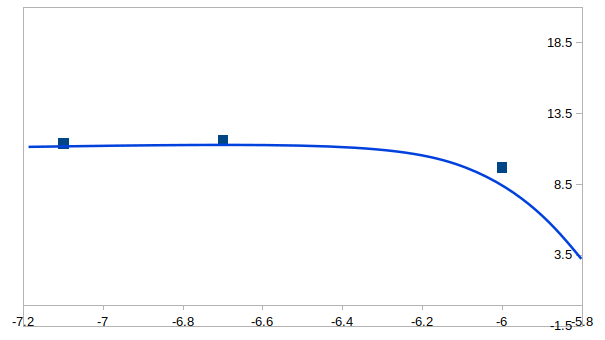
\includegraphics[width=\linewidth]{fig13}
		\caption{\footnotesize{Grafica de los $s_{i}\;vs\;s_{o}$ datos de la tabla \ref{tabla5}.}}
		\label{fig:fig-13}
	\end{Figure} 
Utilizando el cambio de variable  de \ref{ec12} se obtuvo la siguiente ecuación de ajuste
\begin{equation}
	y=-0.6517x-0.0068\implies
\end{equation}
de la ecuación anterior se llega a que $f=86.7\;mm$. El porcentaje de error obtenido es de 
	$$e\%=\dfrac{|-10+8.67|}{10}\times 100=13.23 \%$$
Mientras que usando el cambio de variable de (\ref{ec16}) se obtuvo
\begin{equation}
	y=22.7854x+42.81
\end{equation}
Luego se obtuvo $f=46.9mm$. 
El porcentaje de error obtenido es de 
$$e\%=\dfrac{|-10+4.69|}{10}\times 100= 53.1 \%$$
}	
	\section*{Conclusiones}
	{
		Para el caso en el que las lentes fueron positivas se obtuvieron los resultados esperados, en el caso de las lentes negativas se obtuvieron resultados que no son buenos comparados con los resultados teóricos.
		\\Además en el que las lentes fueron positivas se tenían más datos lo cual implica una mejor precisión en los resultados, mientras que cuando se utilizaron lentes negativas solo se tomaron $3$ datos lo cual influye en la precisión de los resultados.
	}
	
	\medskip
	\\
	\\
	\\
	\\
	\\
	\\
	\\
	\\
	\\
	\\
	\\
	\\
	\\
	\medskip
	\medskip
	\medskip
	\medskip
	\medskip
	\medskip
	
	\nocite{Hecht}\nocite{Rossi}\nocite{Sears}\nocite{Born}\nocite{Tipler}\nocite{Feynman}\nocite{Res}
	\bibliography{miBiblio.bib}
	\bibliographystyle{plain}

\end{multicols}

\end{document}